% Options for packages loaded elsewhere
\PassOptionsToPackage{unicode}{hyperref}
\PassOptionsToPackage{hyphens}{url}
\PassOptionsToPackage{dvipsnames,svgnames,x11names}{xcolor}
%
\documentclass[
  11pt,
  letterpaper,
]{article}
\usepackage{amsmath,amssymb}
\usepackage{iftex}
\ifPDFTeX
  \usepackage[T1]{fontenc}
  \usepackage[utf8]{inputenc}
  \usepackage{textcomp} % provide euro and other symbols
\else % if luatex or xetex
  \usepackage{unicode-math} % this also loads fontspec
  \defaultfontfeatures{Scale=MatchLowercase}
  \defaultfontfeatures[\rmfamily]{Ligatures=TeX,Scale=1}
\fi
\usepackage{lmodern}
\ifPDFTeX\else
  % xetex/luatex font selection
  \setmainfont[]{TeX Gyre Termes}
  \setmonofont[Scale=0.82]{DejaVu Sans Mono}
\fi
% Use upquote if available, for straight quotes in verbatim environments
\IfFileExists{upquote.sty}{\usepackage{upquote}}{}
\IfFileExists{microtype.sty}{% use microtype if available
  \usepackage[]{microtype}
  \UseMicrotypeSet[protrusion]{basicmath} % disable protrusion for tt fonts
}{}
\makeatletter
\@ifundefined{KOMAClassName}{% if non-KOMA class
  \IfFileExists{parskip.sty}{%
    \usepackage{parskip}
  }{% else
    \setlength{\parindent}{0pt}
    \setlength{\parskip}{6pt plus 2pt minus 1pt}}
}{% if KOMA class
  \KOMAoptions{parskip=half}}
\makeatother
\usepackage{xcolor}
\usepackage[margin=2.4cm]{geometry}
\usepackage{longtable,booktabs,array}
\usepackage{calc} % for calculating minipage widths
% Correct order of tables after \paragraph or \subparagraph
\usepackage{etoolbox}
\makeatletter
\patchcmd\longtable{\par}{\if@noskipsec\mbox{}\fi\par}{}{}
\makeatother
% Allow footnotes in longtable head/foot
\IfFileExists{footnotehyper.sty}{\usepackage{footnotehyper}}{\usepackage{footnote}}
\makesavenoteenv{longtable}
\usepackage{graphicx}
\makeatletter
\def\maxwidth{\ifdim\Gin@nat@width>\linewidth\linewidth\else\Gin@nat@width\fi}
\def\maxheight{\ifdim\Gin@nat@height>\textheight\textheight\else\Gin@nat@height\fi}
\makeatother
% Scale images if necessary, so that they will not overflow the page
% margins by default, and it is still possible to overwrite the defaults
% using explicit options in \includegraphics[width, height, ...]{}
\setkeys{Gin}{width=\maxwidth,height=\maxheight,keepaspectratio}
% Set default figure placement to htbp
\makeatletter
\def\fps@figure{htbp}
\makeatother
\setlength{\emergencystretch}{3em} % prevent overfull lines
\providecommand{\tightlist}{%
  \setlength{\itemsep}{0pt}\setlength{\parskip}{0pt}}
\setcounter{secnumdepth}{5}
\ifLuaTeX
\usepackage[bidi=basic]{babel}
\else
\usepackage[bidi=default]{babel}
\fi
\babelprovide[main,import]{spanish}
\ifPDFTeX
\else
\babelfont{rm}[]{TeX Gyre Termes}
\fi
% get rid of language-specific shorthands (see #6817):
\let\LanguageShortHands\languageshorthands
\def\languageshorthands#1{}
\usepackage{etoolbox}
\usepackage{xcolor}
\definecolor{azul}{HTML}{1F3A5F}
\usepackage{fancyhdr}
\pagestyle{fancy}
\fancyhf{}
\fancyhead[L]{\small\textcolor{azul}{SIMTELE-RISK · Semana 1}}
\fancyhead[R]{\small\textcolor{azul}{Métodos Numéricos · UMSA, FCPN}}
\fancyfoot[C]{\small\thepage}
\renewcommand{\headrulewidth}{0.3pt}
\usepackage{titlesec}
\titleformat{\section}{\Large\bfseries\color{azul}}{\thesection}{0.6em}{}
\titleformat{\subsection}{\large\bfseries\color{azul}}{\thesubsection}{0.6em}{}
\titlespacing*{\section}{0pt}{16pt}{6pt}
\titlespacing*{\subsection}{0pt}{12pt}{4pt}
\usepackage{caption}
\captionsetup{font=small,labelfont=bf,labelsep=period}
\AtBeginEnvironment{longtable}{\small\renewcommand{\arraystretch}{1.2}}
\setlength{\parskip}{4pt plus 1pt}
\setlength{\parindent}{0pt}
\usepackage{float}
\floatplacement{figure}{H}
\ifLuaTeX
  \usepackage{selnolig}  % disable illegal ligatures
\fi
\IfFileExists{bookmark.sty}{\usepackage{bookmark}}{\usepackage{hyperref}}
\IfFileExists{xurl.sty}{\usepackage{xurl}}{} % add URL line breaks if available
\urlstyle{same}
\hypersetup{
  pdflang={es},
  colorlinks=true,
  linkcolor={azul},
  filecolor={Maroon},
  citecolor={Blue},
  urlcolor={azul},
  pdfcreator={LaTeX via pandoc}}

\author{}
\date{}

\begin{document}

\begin{titlepage}
\centering
{\large\bfseries UNIVERSIDAD MAYOR DE SAN ANDRÉS\par}
\vspace{2pt}
{\normalsize Facultad de Ciencias Puras y Naturales\par}
{\normalsize Carrera de Informática\par}
\vspace{1.2cm}
{\normalsize\scshape Métodos Numéricos\par}
\vspace{1.4cm}
{\fontsize{34}{40}\selectfont\bfseries\color{azul} SIMTELE-RISK\par}
\vspace{4pt}
{\Large Desafío integrador final\par}
\vspace{1.0cm}
\rule{0.6\textwidth}{0.6pt}\par
\vspace{0.5cm}
{\large\bfseries Informe de avance, semana 1\par}
\vspace{2pt}
{\large Modelos, teoría de errores y sistemas lineales\par}
\vspace{0.5cm}
\rule{0.6\textwidth}{0.6pt}\par
\vspace{1.4cm}
{\large\bfseries Integrantes\par}
\vspace{6pt}
{\small
\renewcommand{\arraystretch}{1.35}
\begin{tabular}{@{}rlccl@{}}
\toprule
 & \textbf{Nombre} & \textbf{CI} & \textbf{RU} & \textbf{Mención}\\
\midrule
1. & Saúl Walter Callisaya Sumi & 15074779 & 1885982 & Ingeniería de Sistemas\\
2. & Ignacio Josue Zarate Camargo & 12392989 & 1886051 & IA y Ciencia de Datos\\
3. & Luis Alejandro Zeballos Quiroz & 12896709 & 1886052 & IA y Ciencia de Datos\\
4. & Jhoel Percy González Herrera & 9990880 & 1886116 & Ingeniería de Sistemas\\
\bottomrule
\end{tabular}\par}
\vfill
{\small La Paz, Bolivia · noviembre de 2026\par}
\vspace{6pt}
{\footnotesize\itshape Contexto académico inspirado en Mi Teleférico, La Paz. Los escenarios son hipotéticos y los datos sintéticos: no describen fallas verificadas de la empresa ni tienen conexión con equipos reales.\par}
\end{titlepage}
\setcounter{page}{1}

\hypertarget{alcance-entregado}{%
\section{Alcance entregado}\label{alcance-entregado}}

Este informe documenta el avance de la semana 1 de SIMTELE-RISK, la
plataforma web con cuatro casos de estudio de un sistema de transporte
por cable. Cubre el planteamiento de los cuatro modelos, la teoría de
errores transversal y los métodos de sistemas lineales, con ejemplos
manuales, soluciones de referencia y tablas de error.

\begin{longtable}[]{@{}
  >{\raggedright\arraybackslash}p{(\columnwidth - 4\tabcolsep) * \real{0.4409}}
  >{\raggedright\arraybackslash}p{(\columnwidth - 4\tabcolsep) * \real{0.0968}}
  >{\raggedright\arraybackslash}p{(\columnwidth - 4\tabcolsep) * \real{0.4624}}@{}}
\toprule\noalign{}
\begin{minipage}[b]{\linewidth}\raggedright
Compromiso de la semana 1
\end{minipage} & \begin{minipage}[b]{\linewidth}\raggedright
Estado
\end{minipage} & \begin{minipage}[b]{\linewidth}\raggedright
Evidencia
\end{minipage} \\
\midrule\noalign{}
\endhead
\bottomrule\noalign{}
\endlastfoot
Planteamiento de los 4 casos y relación entre modelos y métodos & Hecho
& Sección 2; \texttt{backend/simtele/modulos.py} \\
Teoría de errores transversal & Hecho & Sección 3;
\texttt{numerico/errores.py} \\
Jacobi, Gauss-Seidel, LU, gradiente conjugado y referencia directa &
Hecho & Sección 4; \texttt{numerico/sistemas.py} \\
Pruebas de los 3 escenarios en un caso y definición en los otros & Hecho
& Módulo 2 ejecutado; módulos 1, 3 y 4 definidos (sección 2.2) \\
Prototipo web con 4 módulos, DER inicial y repositorio con README &
Hecho & Secciones 5 y 6; \texttt{frontend/},
\texttt{database/schema.sql} \\
\end{longtable}

\hypertarget{planteamiento-de-los-cuatro-casos}{%
\section{Planteamiento de los cuatro
casos}\label{planteamiento-de-los-cuatro-casos}}

\hypertarget{modelos}{%
\subsection{Modelos matemáticos}\label{modelos}}

\textbf{Módulo 1: detención de emergencia.} Pregunta: ¿cómo varían el
tiempo y la distancia de detención ante cambios de velocidad, tiempo de
reacción y frenado? El modelo es un sistema de EDO con condiciones
iniciales:

\[\frac{dx}{dt}=v,\qquad \frac{dv}{dt}=-a(v,t),\qquad x(0)=0,\quad v(0)=v_0,\qquad v(t_{\mathrm{det}})=0 .\]

Variables: \(x\) posición {[}m{]}, \(v\) velocidad {[}m/s{]}, \(a\)
desaceleración {[}m/s²{]}, \(t_r\) tiempo de reacción {[}s{]}, masa
\(m=1200\) kg. Hipótesis: masa puntual, recorrido rectilíneo y reacción
a velocidad constante. Con desaceleración constante hay solución
analítica de referencia:

\[v(t)=v_0-at,\qquad x(t)=v_0t-\frac{a}{2}t^2,\qquad t_{\mathrm{det}}=\frac{v_0}{a},\qquad d_{\mathrm{fren}}=\frac{v_0^{2}}{2a},\qquad d_{\mathrm{total}}=v_0t_r+\frac{v_0^{2}}{2a}.\]

\emph{Ejemplo manual (escenario NORMAL):} con \(v_0=5\) m/s, \(a=2.5\)
m/s² y \(t_r=0.5\) s resulta \(t_{\mathrm{det}}=5/2.5=2\) s,
\(d_{\mathrm{fren}}=25/5=5\) m y \(d_{\mathrm{total}}=2.5+5=7.5\) m.
Métodos previstos: Heun (RK2) y RK4 para la EDO; bisección,
Newton-Raphson y secante para \(v(t)=0\); trapecio, Simpson 1/3 y
Romberg para \(\int_0^{t_{\mathrm{det}}}v\,dt\).

\textbf{Módulo 2: deterioro y mantenimiento.} Pregunta: ¿cuándo
alcanzaría un indicador hipotético de deterioro un umbral de inspección?
El indicador y la condición de umbral son

\[D(t)=D_0+\alpha t+\beta t^{2},\qquad D(t)-D_u=0 .\]

Variables: \(D\) desgaste hipotético {[}\%{]}, \(t\) tiempo {[}meses{]},
\(\alpha\) {[}\%/mes{]}, \(\beta\) {[}\%/mes²{]}. Si \(\alpha,\beta>0\)
y \(D_0<D_u\), el producto de las raíces \((D_0-D_u)/\beta\) es
negativo, de modo que hay una única raíz positiva físicamente admisible:

\[t^{*}=\frac{-\alpha+\sqrt{\alpha^{2}-4\beta\,(D_0-D_u)}}{2\beta}.\]

Los coeficientes se calibran resolviendo \(A\mathbf{x}=\mathbf{b}\) con
\(A\) simétrica definida positiva (SPD) y \(\mathbf{b}=A\mathbf{x}^{*}\)
para una \(\mathbf{x}^{*}\) conocida, lo que permite comparar Jacobi,
Gauss-Seidel, LU y gradiente conjugado contra la solución exacta. Este
es el módulo cuyos tres escenarios se ejecutan en esta entrega (sección
4).

\textbf{Módulo 3: oscilaciones por viento.} Pregunta: ¿cómo cambia la
oscilación ante variaciones de fuerza externa, amortiguamiento y
parámetros? El oscilador lineal de un grado de libertad y su forma de
primer orden son

\[m\,x''+c\,x'+k\,x=F(t)\quad\Longleftrightarrow\quad x'=v,\qquad v'=\frac{F(t)-c\,v-k\,x}{m},\qquad I=\int_0^{T}x(t)^{2}\,dt .\]

Variables: \(x\) {[}m{]}, \(v\) {[}m/s{]}, \(m\) {[}kg{]}, \(k\)
{[}N/m{]}, \(c\) {[}N·s/m{]}, \(F\) {[}N{]}. Con \(F=0\) y régimen
subamortiguado (\(0<\zeta<1\)) la referencia analítica es

\[x(t)=e^{-\zeta\omega_0 t}\left[C_1\cos(\omega_d t)+C_2\sin(\omega_d t)\right],\qquad \omega_0=\sqrt{\tfrac{k}{m}},\quad \zeta=\frac{c}{2\sqrt{km}},\quad \omega_d=\omega_0\sqrt{1-\zeta^{2}} .\]

\emph{Ejemplo manual (NORMAL):} con \(m=1200\) kg y \(k=4800\) N/m,
\(\omega_0=\sqrt{4}=2\) rad/s; con \(\zeta=0.05\) se obtiene
\(c=2\zeta\sqrt{km}=240\) N·s/m y
\(\omega_d=2\sqrt{1-0.0025}\approx 1.9975\) rad/s. Métodos previstos:
Heun y RK4 para la EDO; trapecio, Simpson 1/3 y Romberg para \(I\).

\textbf{Módulo 4: reconstrucción de señales de sensores.} Pregunta:
¿cómo reconstruir registros faltantes y medir la distorsión que produce
el ruido? Dado \(y(t)\) conocida en \(N\) instantes, se ocultan puntos
de prueba \(t_h\) y se mide \(e=|p(t_h)-y(t_h)|\), donde \(p\) interpola
los nodos restantes. Para el polinomio de Lagrange,

\[p_n(t)=\sum_{i=0}^{n}y_i\,L_i(t),\qquad L_i(t)=\prod_{j\neq i}\frac{t-t_j}{t_i-t_j},\qquad y(t)-p_n(t)=\frac{y^{(n+1)}(\xi)}{(n+1)!}\prod_{i=0}^{n}(t-t_i).\]

El factor \(\prod(t-t_i)\) explica por qué nodos equiespaciados pueden
ser desfavorables (fenómeno de Runge). Variables: \(t\) {[}s{]}, \(y\)
señal normalizada {[}u{]}, \(\sigma\) ruido {[}u{]}. Hipótesis: señal
sintética conocida y ruido gaussiano con semilla fija. Métodos:
Lagrange, Newton por diferencias divididas y spline cúbico natural.

\hypertarget{escenarios}{%
\subsection{Matriz de escenarios}\label{escenarios}}

Cada módulo se ejecutará en las tres condiciones. Los parámetros están
definidos desde ahora para que los experimentos sean reproducibles.

\begin{longtable}[]{@{}
  >{\raggedright\arraybackslash}p{(\columnwidth - 6\tabcolsep) * \real{0.1735}}
  >{\raggedright\arraybackslash}p{(\columnwidth - 6\tabcolsep) * \real{0.2755}}
  >{\raggedright\arraybackslash}p{(\columnwidth - 6\tabcolsep) * \real{0.2755}}
  >{\raggedright\arraybackslash}p{(\columnwidth - 6\tabcolsep) * \real{0.2755}}@{}}
\toprule\noalign{}
\begin{minipage}[b]{\linewidth}\raggedright
Módulo
\end{minipage} & \begin{minipage}[b]{\linewidth}\raggedright
NORMAL
\end{minipage} & \begin{minipage}[b]{\linewidth}\raggedright
ESTRÉS
\end{minipage} & \begin{minipage}[b]{\linewidth}\raggedright
MAL CONDICIONADO
\end{minipage} \\
\midrule\noalign{}
\endhead
\bottomrule\noalign{}
\endlastfoot
Detención (M1) & \(v_0=5\) m/s, \(a=2.5\) m/s², \(t_r=0.5\) s, \(h=0.1\)
s & \(v_0=7\) m/s, \(a=1.2+0.05v^{2}\), \(t_r=1.5\) s, \(h=0.5\) s, tol
\(=10^{-13}\) & Frenado plano \(v=v_0(1-t/T)^{5}\): raíz múltiple con
derivada nula \\
Deterioro (M2) & \(A=I+0.1L\), \(n=6\), tol \(=10^{-10}\) & \(A=I+5L\),
\(n=40\), tol \(=10^{-12}\) & Hilbert \(n=8\); curva casi tangente al
umbral \\
Oscilaciones (M3) & Vibración libre, \(\zeta=0.05\), \(h=0.05\) s &
Ráfaga armónica \(F_0=1500\) N cerca de resonancia, \(h=0.5\) s &
\(\zeta=0.005\) en el flanco de la resonancia \\
Sensores (M4) & \(y=\sin t\), 17 muestras, sin ruido & Senoidal
amortiguada, 31 muestras, \(\sigma=0.002\) & Pulso de Runge, 21 nodos
uniformes \\
\end{longtable}

Un escenario mal condicionado es un subexperimento numérico: se
distingue de ESTRÉS (condiciones más exigentes) y de un fallo de
convergencia (propiedad de un método sobre un problema). No toda
situación físicamente peligrosa es matemáticamente mal condicionada.

\hypertarget{teoruxeda-de-errores-transversal}{%
\section{Teoría de errores
transversal}\label{teoruxeda-de-errores-transversal}}

La teoría de errores se aplica a todas las familias de métodos y a los
cuatro módulos. Sea \(x_{\mathrm{ref}}\) el valor de referencia y \(x\)
el aproximado.

\begin{longtable}[]{@{}
  >{\raggedright\arraybackslash}p{(\columnwidth - 4\tabcolsep) * \real{0.1765}}
  >{\raggedright\arraybackslash}p{(\columnwidth - 4\tabcolsep) * \real{0.5294}}
  >{\raggedright\arraybackslash}p{(\columnwidth - 4\tabcolsep) * \real{0.2941}}@{}}
\toprule\noalign{}
\begin{minipage}[b]{\linewidth}\raggedright
Medida
\end{minipage} & \begin{minipage}[b]{\linewidth}\raggedright
Fórmula
\end{minipage} & \begin{minipage}[b]{\linewidth}\raggedright
Aplicación
\end{minipage} \\
\midrule\noalign{}
\endhead
\bottomrule\noalign{}
\endlastfoot
Error absoluto & \(E_a=\lvert x_{\mathrm{ref}}-x\rvert\); vectorial
\(\lVert \mathbf{x}_{\mathrm{ref}}-\mathbf{x}\rVert_2\) & Todos los
módulos \\
Error relativo & \(E_r=E_a/\lvert x_{\mathrm{ref}}\rvert\) (se omite si
\(x_{\mathrm{ref}}=0\)) & Todos los módulos \\
Error porcentual & \(E_{\%}=100\,E_r\) & Tablas de resultados \\
Residual &
\(\lVert \mathbf{b}-A\mathbf{x}\rVert_2/\lVert \mathbf{b}\rVert_2\);
\(\lvert f(x)\rvert\) en raíces & Sistemas, raíces \\
Sensibilidad &
\(\kappa_{\mathrm{rel}}=\dfrac{\lvert\delta S/S\rvert}{\lvert\delta E/E\rvert}\)
(perturbación finita de la entrada) & Perturbaciones en todos los
módulos \\
Orden observado & \(p=\dfrac{\ln(e_h/e_{h/r})}{\ln r}\) & EDO e
integración \\
\end{longtable}

\emph{Ejemplo manual:} si \(x_{\mathrm{ref}}=2\) y \(x=1.5\), entonces
\(E_a=0.5\), \(E_r=0.25\) y \(E_{\%}=25\,\%\).

Para sistemas lineales, el número de condición
\(\kappa(A)=\lVert A\rVert\,\lVert A^{-1}\rVert\) acota cuánto se
amplifican las perturbaciones y relaciona el residuo con el error:

\[\frac{\lVert \delta\mathbf{x}\rVert}{\lVert \mathbf{x}\rVert}\le\kappa(A)\,\frac{\lVert \delta\mathbf{b}\rVert}{\lVert \mathbf{b}\rVert},\qquad\qquad \frac{\lVert \mathbf{x}-\mathbf{x}^{*}\rVert}{\lVert \mathbf{x}^{*}\rVert}\le\kappa(A)\,\frac{\lVert \mathbf{b}-A\mathbf{x}\rVert}{\lVert \mathbf{b}\rVert}.\]

Por eso un residuo pequeño no garantiza un error pequeño cuando
\(\kappa(A)\) es grande (sección 4.5).

\hypertarget{sistemas}{%
\section{Sistemas lineales}\label{sistemas}}

\hypertarget{muxe9todos-y-condiciones-de-convergencia}{%
\subsection{Métodos y condiciones de
convergencia}\label{muxe9todos-y-condiciones-de-convergencia}}

Sea \(A=L+D+U\) con \(D\) la diagonal, \(L\) la parte estrictamente
triangular inferior y \(U\) la superior.

\[\text{Jacobi:}\quad x_i^{(k+1)}=\frac{1}{a_{ii}}\left(b_i-\sum_{j\neq i}a_{ij}\,x_j^{(k)}\right)\]

\[\text{Gauss-Seidel:}\quad x_i^{(k+1)}=\frac{1}{a_{ii}}\left(b_i-\sum_{j<i}a_{ij}\,x_j^{(k+1)}-\sum_{j>i}a_{ij}\,x_j^{(k)}\right)\]

\[\text{LU con pivoteo:}\quad PA=LU,\qquad L\mathbf{z}=P\mathbf{b},\qquad U\mathbf{x}=\mathbf{z}\]

\[\text{Gradiente conjugado:}\quad \alpha_k=\frac{\mathbf{r}_k^{\top}\mathbf{r}_k}{\mathbf{p}_k^{\top}A\mathbf{p}_k},\quad \mathbf{x}_{k+1}=\mathbf{x}_k+\alpha_k\mathbf{p}_k,\quad \mathbf{r}_{k+1}=\mathbf{r}_k-\alpha_kA\mathbf{p}_k,\quad \mathbf{p}_{k+1}=\mathbf{r}_{k+1}+\frac{\mathbf{r}_{k+1}^{\top}\mathbf{r}_{k+1}}{\mathbf{r}_k^{\top}\mathbf{r}_k}\,\mathbf{p}_k\]

Condiciones de convergencia que se justifican en cada experimento:

\begin{itemize}
\tightlist
\item
  \textbf{Jacobi} converge si y solo si \(\rho(T_J)<1\), con
  \(T_J=I-D^{-1}A\). Que \(A\) sea SPD no basta.
\item
  \textbf{Gauss-Seidel} converge para toda matriz SPD; en general
  converge si y solo si \(\rho(T_{GS})<1\).
\item
  \textbf{Gradiente conjugado} exige \(A\) SPD. En aritmética exacta
  termina en a lo sumo \(n\) pasos y cumple
  \(\lVert \mathbf{e}_k\rVert_A\le 2\left(\tfrac{\sqrt{\kappa}-1}{\sqrt{\kappa}+1}\right)^{k}\lVert \mathbf{e}_0\rVert_A\).
\item
  \textbf{Criterio de parada} de los iterativos:
  \(\lVert \mathbf{b}-A\mathbf{x}_k\rVert_2/\lVert \mathbf{b}\rVert_2\le\mathrm{tol}\),
  con tope de iteraciones y detección de divergencia
  (\(\lVert \mathbf{x}\rVert>10^{100}\)).
\end{itemize}

\hypertarget{manual}{%
\subsection{Ejemplo manual de 4 × 4}\label{manual}}

\[A=\begin{bmatrix}4&1&0&0\\1&4&1&0\\0&1&4&1\\0&0&1&4\end{bmatrix},\qquad \mathbf{x}^{*}=\begin{bmatrix}1\\-2\\3\\0.5\end{bmatrix},\qquad \mathbf{b}=A\mathbf{x}^{*}=\begin{bmatrix}2\\-4\\10.5\\5\end{bmatrix},\qquad \kappa_2(A)=2.359 .\]

Comprobación de \(\mathbf{b}\): fila 1, \(4(1)+1(-2)=2\); fila 2,
\(1+4(-2)+3=-4\); fila 3, \(-2+4(3)+0.5=10.5\); fila 4, \(3+4(0.5)=5\).

\textbf{Primer barrido desde \(\mathbf{x}^{(0)}=\mathbf{0}\).}

\begin{longtable}[]{@{}
  >{\raggedright\arraybackslash}p{(\columnwidth - 10\tabcolsep) * \real{0.1263}}
  >{\raggedright\arraybackslash}p{(\columnwidth - 10\tabcolsep) * \real{0.1263}}
  >{\raggedright\arraybackslash}p{(\columnwidth - 10\tabcolsep) * \real{0.2105}}
  >{\raggedright\arraybackslash}p{(\columnwidth - 10\tabcolsep) * \real{0.2421}}
  >{\raggedright\arraybackslash}p{(\columnwidth - 10\tabcolsep) * \real{0.2105}}
  >{\raggedright\arraybackslash}p{(\columnwidth - 10\tabcolsep) * \real{0.0842}}@{}}
\toprule\noalign{}
\begin{minipage}[b]{\linewidth}\raggedright
Método
\end{minipage} & \begin{minipage}[b]{\linewidth}\raggedright
\(x_1\)
\end{minipage} & \begin{minipage}[b]{\linewidth}\raggedright
\(x_2\)
\end{minipage} & \begin{minipage}[b]{\linewidth}\raggedright
\(x_3\)
\end{minipage} & \begin{minipage}[b]{\linewidth}\raggedright
\(x_4\)
\end{minipage} & \begin{minipage}[b]{\linewidth}\raggedright
\(\lVert \mathbf{x}-\mathbf{x}^{*}\rVert_2\)
\end{minipage} \\
\midrule\noalign{}
\endhead
\bottomrule\noalign{}
\endlastfoot
Jacobi & \(2/4=0.5\) & \(-4/4=-1\) & \(10.5/4=2.625\) & \(5/4=1.25\) &
1.398 \\
Gauss-Seidel & \(2/4=0.5\) & \((-4-0.5)/4=-1.125\) &
\((10.5+1.125)/4=2.90625\) & \((5-2.90625)/4=0.5234\) & 1.012 \\
\end{longtable}

\textbf{LU sin intercambios.} Los multiplicadores y pivotes son
\(l_{21}=0.25\), \(u_{22}=3.75\), \(l_{32}=0.26667\),
\(u_{33}=3.73333\), \(l_{43}=0.26786\), \(u_{44}=3.73214\). Con
\(L\mathbf{z}=\mathbf{b}\) se obtiene
\(\mathbf{z}=(2,\,-4.5,\,11.7,\,1.86607)^{\top}\). Sustituyendo hacia
atrás en \(U\mathbf{x}=\mathbf{z}\): \(x_4=0.5\), \(x_3=3\), \(x_2=-2\),
\(x_1=1\), que coincide con \(\mathbf{x}^{*}\).

\textbf{Gradiente conjugado, primer paso.}
\(\mathbf{r}_0=\mathbf{p}_0=\mathbf{b}\),
\(\mathbf{r}_0^{\top}\mathbf{r}_0=155.25\),
\(A\mathbf{b}=(4,\,-3.5,\,43,\,30.5)^{\top}\) y
\(\mathbf{p}_0^{\top}A\mathbf{p}_0=626\). Entonces
\(\alpha_0=155.25/626=0.2480\) y
\(\mathbf{x}_1=(0.4960,\,-0.9920,\,2.6040,\,1.2400)^{\top}\).

La prueba \texttt{backend/tests/test\_semana1.py} verifica los barridos
de Jacobi y Gauss-Seidel, la factorización LU y la solución exacta.

\hypertarget{matrices-de-referencia-del-muxf3dulo-2}{%
\subsection{Matrices de referencia del módulo
2}\label{matrices-de-referencia-del-muxf3dulo-2}}

\begin{itemize}
\tightlist
\item
  \textbf{NORMAL y ESTRÉS:} \(A=I+\lambda L\), donde \(L\) es el
  laplaciano de un camino de \(n\) tramos (1 en los dos extremos de la
  diagonal y 2 en el resto, \(-1\) entre vecinos). Es SPD con
  autovalores en \([1,\,1+4\lambda)\). La solución prefijada es
  \(x_i^{*}=20+10\sin(2\pi i/n)\) con \(i=0,\dots,n-1\) (desgaste
  hipotético en \%).
\item
  \textbf{MAL CONDICIONADO:} matriz de Hilbert
  \(H_{ij}=\dfrac{1}{i+j+1}\), \(i,j=0,\dots,n-1\), que es la matriz de
  Gram de la base monomial en \([0,1]\) (SPD), con
  \(\mathbf{x}^{*}=(1,\dots,1)^{\top}\).
\end{itemize}

En todos los casos \(\mathbf{b}=A\mathbf{x}^{*}\).

\hypertarget{resultados}{%
\subsection{Resultados por escenario}\label{resultados}}

Se generan con \texttt{python\ -m\ backend.simtele.experimentos}. Los
indicadores del sistema son:

\begin{longtable}[]{@{}
  >{\raggedright\arraybackslash}p{(\columnwidth - 12\tabcolsep) * \real{0.1818}}
  >{\raggedright\arraybackslash}p{(\columnwidth - 12\tabcolsep) * \real{0.0455}}
  >{\raggedright\arraybackslash}p{(\columnwidth - 12\tabcolsep) * \real{0.1667}}
  >{\raggedright\arraybackslash}p{(\columnwidth - 12\tabcolsep) * \real{0.1212}}
  >{\raggedright\arraybackslash}p{(\columnwidth - 12\tabcolsep) * \real{0.1212}}
  >{\raggedright\arraybackslash}p{(\columnwidth - 12\tabcolsep) * \real{0.1212}}
  >{\raggedright\arraybackslash}p{(\columnwidth - 12\tabcolsep) * \real{0.2424}}@{}}
\toprule\noalign{}
\begin{minipage}[b]{\linewidth}\raggedright
Escenario
\end{minipage} & \begin{minipage}[b]{\linewidth}\raggedright
\(n\)
\end{minipage} & \begin{minipage}[b]{\linewidth}\raggedright
\(\kappa_2(A)\)
\end{minipage} & \begin{minipage}[b]{\linewidth}\raggedright
\(\rho(T_J)\)
\end{minipage} & \begin{minipage}[b]{\linewidth}\raggedright
\(\rho(T_{GS})\)
\end{minipage} & \begin{minipage}[b]{\linewidth}\raggedright
tol
\end{minipage} & \begin{minipage}[b]{\linewidth}\raggedright
Amplificación máxima medida de \(\delta\mathbf{b}\) en \(\mathbf{x}\)
\end{minipage} \\
\midrule\noalign{}
\endhead
\bottomrule\noalign{}
\endlastfoot
NORMAL & 6 & 1.373 & 0.1516 & 0.0230 & \(10^{-10}\) & 1.009 \\
ESTRÉS & 40 & 20.97 & 0.9078 & 0.8241 & \(10^{-12}\) & 1.017 \\
MAL CONDICIONADO & 8 & \(1.526\times10^{10}\) & 6.042 & 1.000 &
\(10^{-10}\) & \(1.319\times10^{10}\) \\
\end{longtable}

\begin{longtable}[]{@{}
  >{\raggedright\arraybackslash}p{(\columnwidth - 12\tabcolsep) * \real{0.1047}}
  >{\raggedright\arraybackslash}p{(\columnwidth - 12\tabcolsep) * \real{0.2326}}
  >{\raggedright\arraybackslash}p{(\columnwidth - 12\tabcolsep) * \real{0.0930}}
  >{\raggedright\arraybackslash}p{(\columnwidth - 12\tabcolsep) * \real{0.1512}}
  >{\raggedright\arraybackslash}p{(\columnwidth - 12\tabcolsep) * \real{0.1395}}
  >{\raggedright\arraybackslash}p{(\columnwidth - 12\tabcolsep) * \real{0.1395}}
  >{\raggedright\arraybackslash}p{(\columnwidth - 12\tabcolsep) * \real{0.1395}}@{}}
\toprule\noalign{}
\begin{minipage}[b]{\linewidth}\raggedright
Escenario
\end{minipage} & \begin{minipage}[b]{\linewidth}\raggedright
Método
\end{minipage} & \begin{minipage}[b]{\linewidth}\raggedright
Iter.
\end{minipage} & \begin{minipage}[b]{\linewidth}\raggedright
¿Convergió?
\end{minipage} & \begin{minipage}[b]{\linewidth}\raggedright
\(\lVert \mathbf{x}-\mathbf{x}^{*}\rVert_2\)
\end{minipage} & \begin{minipage}[b]{\linewidth}\raggedright
Error relativo
\end{minipage} & \begin{minipage}[b]{\linewidth}\raggedright
Residuo relativo
\end{minipage} \\
\midrule\noalign{}
\endhead
\bottomrule\noalign{}
\endlastfoot
NORMAL & Jacobi & 13 & Sí & \(1.106\times10^{-9}\) &
\(2.129\times10^{-11}\) & \(2.127\times10^{-11}\) \\
& Gauss-Seidel & 8 & Sí & \(1.570\times10^{-9}\) &
\(3.022\times10^{-11}\) & \(3.169\times10^{-11}\) \\
& LU con pivoteo parcial & 1 & Sí & \(7.944\times10^{-15}\) &
\(1.529\times10^{-16}\) & \(9.584\times10^{-17}\) \\
& Gradiente conjugado & 5 & Sí & \(8.140\times10^{-15}\) &
\(1.567\times10^{-16}\) & \(1.728\times10^{-16}\) \\
ESTRÉS & Jacobi & 285 & Sí & \(1.326\times10^{-10}\) &
\(9.887\times10^{-13}\) & \(9.799\times10^{-13}\) \\
& Gauss-Seidel & 147 & Sí & \(1.146\times10^{-10}\) &
\(8.545\times10^{-13}\) & \(8.488\times10^{-13}\) \\
& LU con pivoteo parcial & 1 & Sí & \(2.562\times10^{-14}\) &
\(1.910\times10^{-16}\) & \(8.899\times10^{-16}\) \\
& Gradiente conjugado & 22 & Sí & \(3.398\times10^{-14}\) &
\(2.533\times10^{-16}\) & \(2.044\times10^{-15}\) \\
MAL COND. & Jacobi & 128 & No: diverge & \(3.426\times10^{100}\) &
\(1.211\times10^{100}\) & \(9.076\times10^{99}\) \\
& Gauss-Seidel & 5000 & No: máx. iter. & \(3.350\times10^{-2}\) &
\(1.184\times10^{-2}\) & \(2.185\times10^{-7}\) \\
& LU con pivoteo parcial & 1 & Sí & \(3.394\times10^{-7}\) &
\(1.200\times10^{-7}\) & \(2.677\times10^{-17}\) \\
& Gradiente conjugado & 8 & Sí & \(4.236\times10^{-4}\) &
\(1.498\times10^{-4}\) & \(6.903\times10^{-11}\) \\
\end{longtable}

\emph{Nota de reproducibilidad.} El número de iteraciones, \(\kappa_2\),
los radios espectrales y los errores mayores que \(10^{-10}\) se
reproducen exactamente al volver a ejecutar el código. Los valores
cercanos a la precisión de máquina (del orden de \(10^{-15}\) a
\(10^{-17}\)) varían ligeramente entre computadoras según la biblioteca
de álgebra lineal.

\begin{figure}
\centering
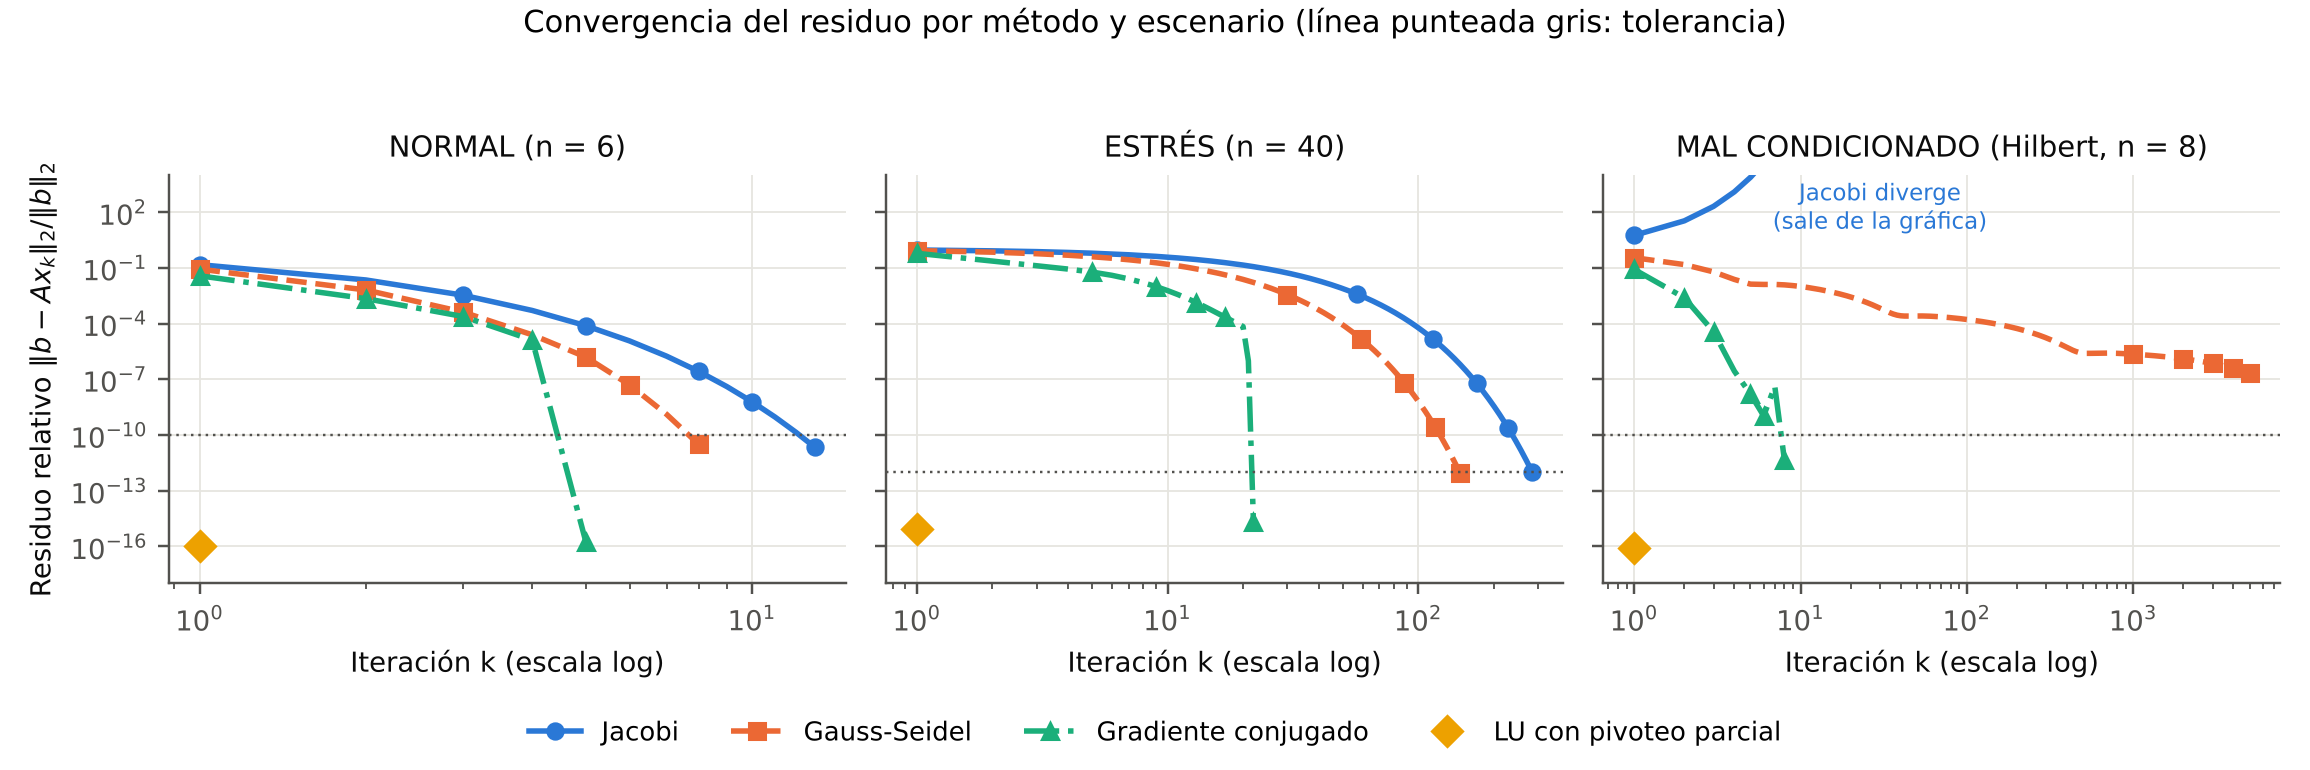
\includegraphics[width=1\textwidth,height=\textheight]{fig/convergencia.png}
\caption{Residuo relativo por iteración de cada método, en los tres
escenarios del módulo 2 (escala log-log).}
\end{figure}

\hypertarget{lectura}{%
\subsection{Lectura de resultados}\label{lectura}}

\begin{itemize}
\tightlist
\item
  \textbf{NORMAL y ESTRÉS.} Gauss-Seidel necesita cerca de la mitad de
  las iteraciones de Jacobi, coherente con
  \(\rho(T_{GS})\approx\rho(T_J)^{2}\) en matrices tridiagonales:
  \(0.1516^{2}=0.0230\) y \(0.9078^{2}=0.8241\). El gradiente conjugado
  es el iterativo más rápido (5 y 22 iteraciones). LU resuelve en un
  solo paso, pero su costo crece como \(\mathcal{O}(n^{3})\), relevante
  para sistemas grandes.
\item
  \textbf{MAL CONDICIONADO, condicionamiento.} LU termina con residuo
  relativo de \(2.7\times10^{-17}\) y error relativo de
  \(1.2\times10^{-7}\): el error es unas \(10^{10}\) veces mayor que el
  residuo, coherente con \(\kappa_2\approx1.5\times10^{10}\) y con la
  cota de la sección 3. Un residuo pequeño no implica una solución
  precisa.
\item
  \textbf{MAL CONDICIONADO, convergencia.} Jacobi diverge porque
  \(\rho(T_J)=6.04>1\): es una propiedad del método sobre esa matriz.
  Gauss-Seidel converge en teoría, pero \(\rho\approx1\) hace que no
  termine en 5000 iteraciones. Ambos fenómenos son distintos del mal
  condicionamiento, que afecta incluso al método directo.
\end{itemize}

\begin{figure}
\centering
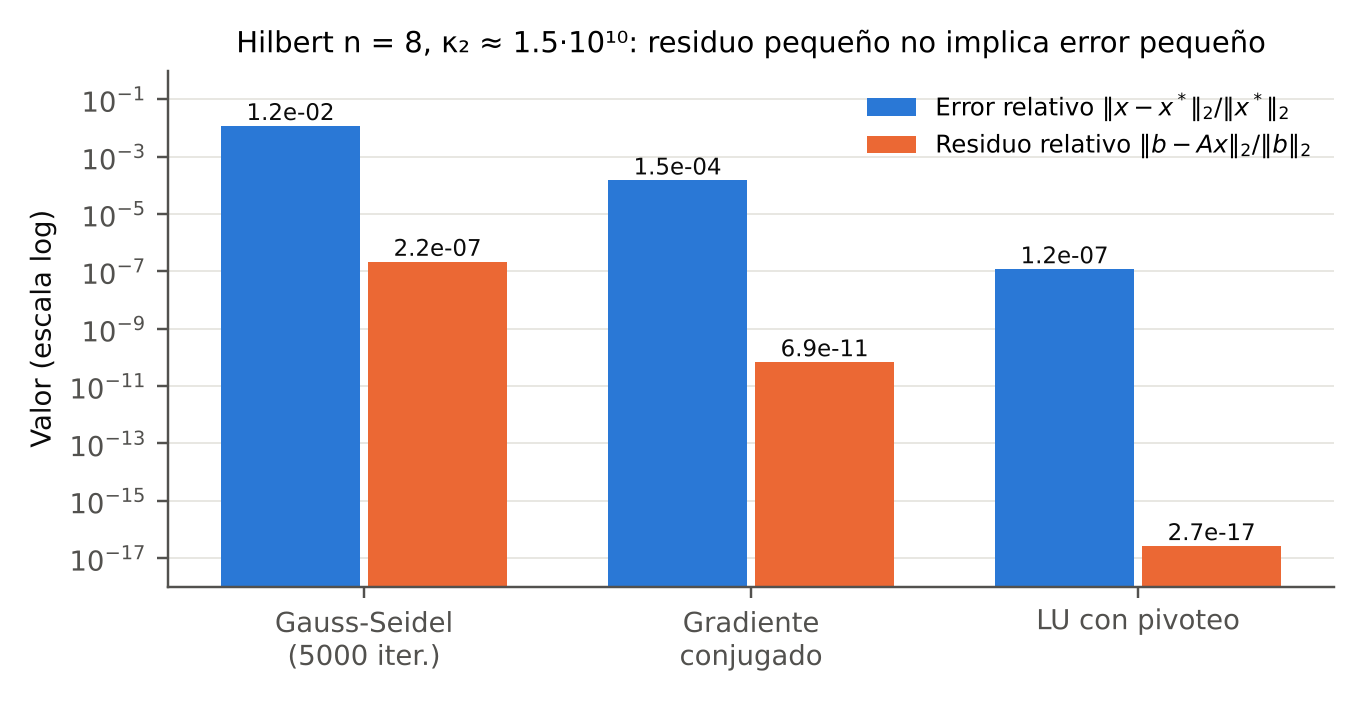
\includegraphics[width=0.75\textwidth,height=\textheight]{fig/error_vs_residuo.png}
\caption{Escenario MAL CONDICIONADO: el residuo es varios órdenes de
magnitud menor que el error en todos los métodos (escala logarítmica).}
\end{figure}

\hypertarget{der}{%
\section{DER inicial y modelo relacional}\label{der}}

El modelo de datos tiene seis entidades, con los campos mínimos de la
consigna. Una ejecución completa queda registrada desde el caso de
estudio hasta cada iteración (figura 3).

\textbf{Modelo relacional} (clave primaria en negrita, clave foránea con
flecha):

\begin{itemize}
\tightlist
\item
  \texttt{caso\_estudio}(\textbf{id}, nombre único, modelo\_version)
\item
  \texttt{escenario}(\textbf{id}, caso\_id → caso\_estudio, tipo,
  parametros\_json, fuente\_datos)
\item
  \texttt{simulacion}(\textbf{id}, escenario\_id → escenario, fecha,
  usuario\_equipo, estado)
\item
  \texttt{ejecucion\_metodo}(\textbf{id}, simulacion\_id → simulacion,
  metodo, tolerancia, paso, max\_iter, convergio, tiempo\_ms)
\item
  \texttt{iteracion\_resultado}(\textbf{id}, ejecucion\_id →
  ejecucion\_metodo, numero, aproximacion\_json, residual, error\_abs,
  error\_rel)
\item
  \texttt{resultado\_resumen}(\textbf{id}, ejecucion\_id único →
  ejecucion\_metodo, referencia, valor\_json, metrica\_error\_json,
  interpretacion)
\end{itemize}

El script \texttt{database/schema.sql} (SQLite 3, con
\texttt{PRAGMA\ foreign\_keys\ =\ ON}) implementa el modelo con
restricciones: \texttt{tipo} solo admite \texttt{NORMAL},
\texttt{ESTRES} o \texttt{MAL\_CONDICIONADO}; \texttt{estado} solo
\texttt{COMPLETADA} o \texttt{FALLIDA}; los campos \texttt{*\_json}
deben ser JSON válido; \texttt{convergio} es 0 o 1; \texttt{tiempo\_ms}
no es negativo. Las claves foráneas usan \texttt{ON\ DELETE\ RESTRICT}
hacia escenarios y simulaciones, y \texttt{ON\ DELETE\ CASCADE} hacia
ejecuciones, iteraciones y resúmenes, además de índices por clave
foránea. La prueba \texttt{database/tests/test\_schema.py} comprueba la
creación y la integridad del esquema. En la semana 3 se conectará la
base con la API para guardar y recuperar ejecuciones completas, incluida
la prueba de reinicio exigida por la consigna.

\begin{figure}
\centering
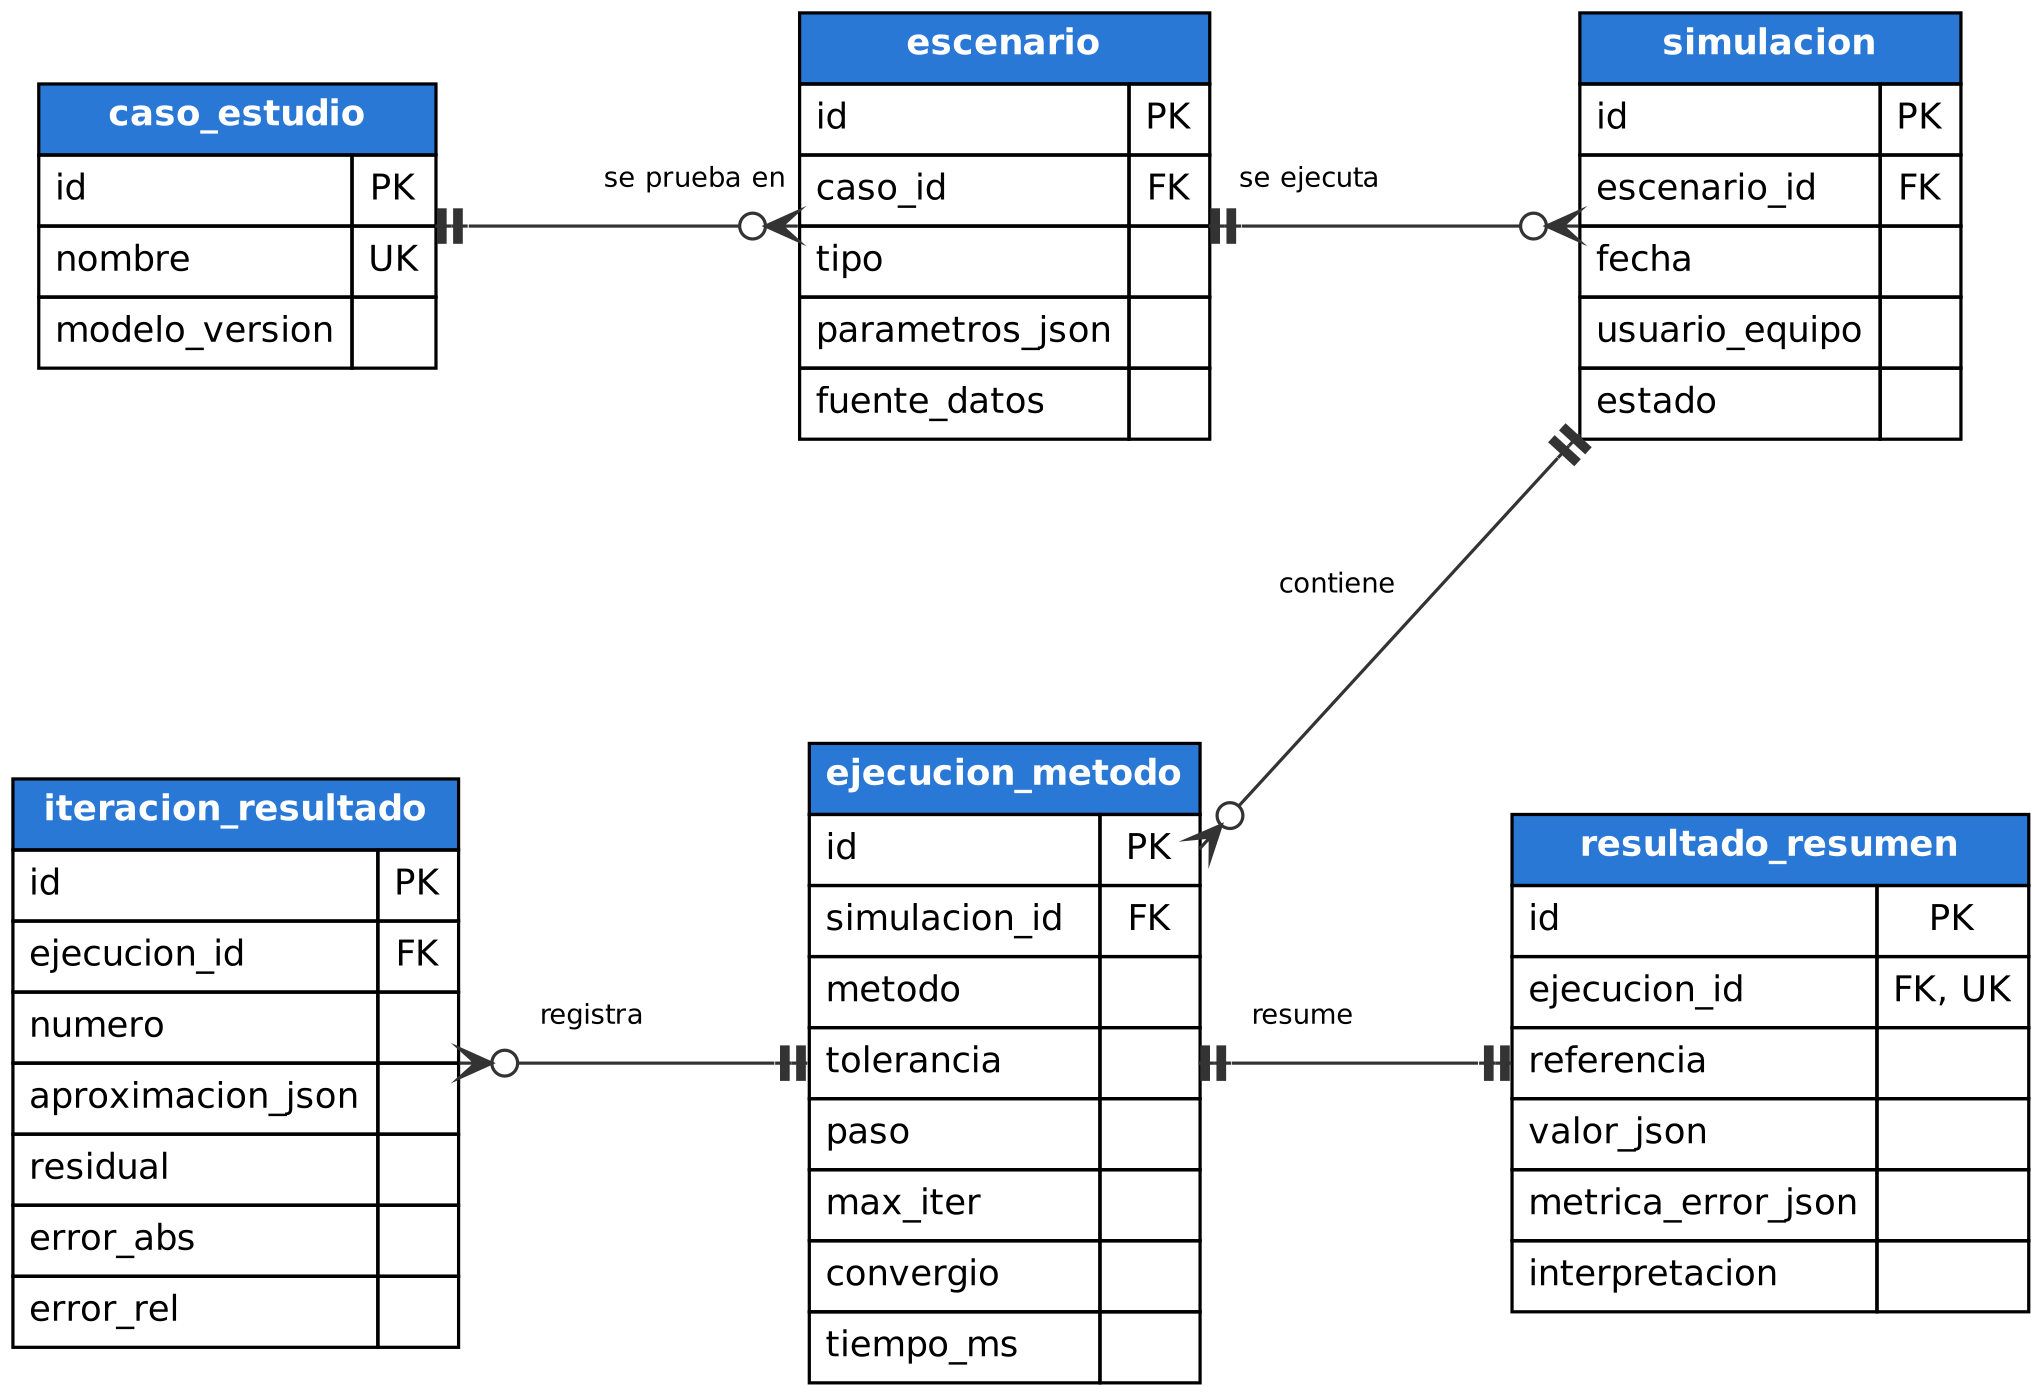
\includegraphics[width=1\textwidth,height=\textheight]{fig/der.png}
\caption{Diagrama entidad-relación inicial de SIMTELE-RISK. Notación de
pata de gallo: un extremo con doble barra es «uno» y el extremo con
círculo y pata es «cero o muchos».}
\end{figure}

\hypertarget{prototipo-web-y-repositorio}{%
\section{Prototipo web y
repositorio}\label{prototipo-web-y-repositorio}}

El prototipo es una página estática (\texttt{frontend/index.html}) con:

\begin{itemize}
\tightlist
\item
  cuatro tarjetas, una por módulo, cada una con su modelo, variables y
  matriz de escenarios;
\item
  el panel del módulo 2 con selector de escenario, indicadores
  (\(\kappa_2\), \(\rho\), amplificación), gráfico de residuo por
  iteración (Chart.js) y tabla de errores con el criterio de parada de
  cada método;
\item
  una burbuja flotante que abre un modal con los integrantes, leídos de
  \texttt{estudiantes.json}.
\end{itemize}

\textbf{Estructura de la entrega}
(\texttt{v1\_semana1\_modelos\_sistemas/}):

\begin{verbatim}
backend/simtele/    modulos.py, experimentos.py, numerico/errores.py, numerico/sistemas.py
backend/tests/      test_semana1.py
database/           schema.sql, tests/test_schema.py
frontend/           index.html, css/, js/, datos/experimentos.json, vendor/chart.umd.js
estudiantes.json    informe_semana1.md    pytest.ini
\end{verbatim}

\textbf{Ejecución,} desde la carpeta de la versión:

\begin{verbatim}
pip install -r backend/requirements.txt
python -m backend.simtele.experimentos
python -m pytest
python -m http.server 8000
\end{verbatim}

Luego se abre \texttt{http://localhost:8000/frontend/}. El servidor se
ejecuta desde la carpeta de la versión para que el modal lea
\texttt{estudiantes.json}. Las pruebas automáticas dan 21 superadas.

\textbf{Repositorio GitHub:}
\url{https://github.com/Saul-C006/desafio-final-metodos}

\hypertarget{menciones}{%
\section{Enfoque por mención}\label{menciones}}

El proyecto se trabaja desde las dos menciones del grupo, sin perder el
dominio común de las bases matemáticas. En la defensa, cada integrante
explicará los aportes desde su mención.

\begin{longtable}[]{@{}
  >{\raggedright\arraybackslash}p{(\columnwidth - 6\tabcolsep) * \real{0.1524}}
  >{\raggedright\arraybackslash}p{(\columnwidth - 6\tabcolsep) * \real{0.1524}}
  >{\raggedright\arraybackslash}p{(\columnwidth - 6\tabcolsep) * \real{0.3905}}
  >{\raggedright\arraybackslash}p{(\columnwidth - 6\tabcolsep) * \real{0.3048}}@{}}
\toprule\noalign{}
\begin{minipage}[b]{\linewidth}\raggedright
Mención
\end{minipage} & \begin{minipage}[b]{\linewidth}\raggedright
Integrantes
\end{minipage} & \begin{minipage}[b]{\linewidth}\raggedright
Enfoque en SIMTELE-RISK
\end{minipage} & \begin{minipage}[b]{\linewidth}\raggedright
Evidencia en la semana 1
\end{minipage} \\
\midrule\noalign{}
\endhead
\bottomrule\noalign{}
\endlastfoot
Ingeniería de Sistemas & Saúl Walter Callisaya Sumi; Jhoel Percy
González Herrera & Arquitectura de la aplicación (backend, frontend y
base de datos), modelo de datos y DER, persistencia y recuperación de
ejecuciones tras reiniciar, pruebas automatizadas, organización del
repositorio y reproducibilidad de los experimentos & \texttt{schema.sql}
y su prueba, prototipo web de cuatro módulos, 21 pruebas automáticas,
estructura por versiones \\
IA y Ciencia de Datos & Ignacio Josue Zarate Camargo; Luis Alejandro
Zeballos Quiroz & Calidad y tratamiento de datos (sintéticos con semilla
fija y ruido controlado), métricas de error y sensibilidad, validación
con puntos ocultos, reconstrucción de señales del módulo 4 y calibración
de parámetros como problema de ajuste & Teoría de errores transversal,
indicadores \(\kappa_2\) y amplificación de perturbaciones, definición
de los escenarios con ruido y de interpolación del módulo 4 \\
\end{longtable}

Un enlace natural entre ambas menciones es la calibración por mínimos
cuadrados: el ajuste de coeficientes conduce a las ecuaciones normales
\(A^{\top}A\,\mathbf{x}=A^{\top}\mathbf{y}\), cuya matriz es SPD cuando
\(A\) tiene rango completo, justamente la condición que exige el
gradiente conjugado. Esto conecta el análisis de datos (mención de IA y
Ciencia de Datos) con la solución eficiente y verificable del sistema
(mención de Ingeniería de Sistemas).

\hypertarget{plan-para-la-semana-3}{%
\section{Plan para la semana 3}\label{plan-para-la-semana-3}}

\begin{enumerate}
\def\labelenumi{\arabic{enumi}.}
\tightlist
\item
  Implementar interpolación (Lagrange, Newton por diferencias divididas
  y spline cúbico), raíces (bisección, Newton-Raphson, secante),
  integración (trapecio, Simpson 1/3 y Romberg) y EDO (Heun y RK4), cada
  una con su prueba analítica.
\item
  Ejecutar al menos el escenario NORMAL en los cuatro módulos, con
  tablas, errores y dos gráficos por módulo, e incorporar ESTRÉS y MAL
  CONDICIONADO.
\item
  Conectar la base de datos con la API y guardar ejecuciones completas,
  con la prueba de guardar, cerrar y recuperar.
\item
  Declarar en el informe que la variante de RK2 utilizada es el método
  de Heun.
\end{enumerate}

\hypertarget{referencias}{%
\section*{Referencias}\label{referencias}}
\addcontentsline{toc}{section}{Referencias}

\begin{itemize}
\tightlist
\item
  Burden, R. L. y Faires, J. D. \emph{Análisis numérico}.
\item
  Chapra, S. C. y Canale, R. P. \emph{Métodos numéricos para
  ingenieros}.
\item
  Golub, G. H. y Van Loan, C. F. \emph{Matrix Computations}.
\end{itemize}

\end{document}
